\documentclass[12pt]{article}
\usepackage{graphicx}
\usepackage{amsmath}
\begin{center}
\textbf{Sushant Virupaksha Bedage}
\end{center}
\hline
\label{sec:SushantVirupakshaBedage}
\begin{document}
\begin{flushleft}
Classic park,\hspace{2.8in} Contact:8805503611\\ 
Kupwad road,\hspace{1in} Email Id:sushantbedage95@gmail.com\\ 
Vishrambag,\\ 
Sangli-416416,\\ 
Maharashtra.
\vspace{-4ex}
\begin{figure}[h]
	\begin{flushright}
		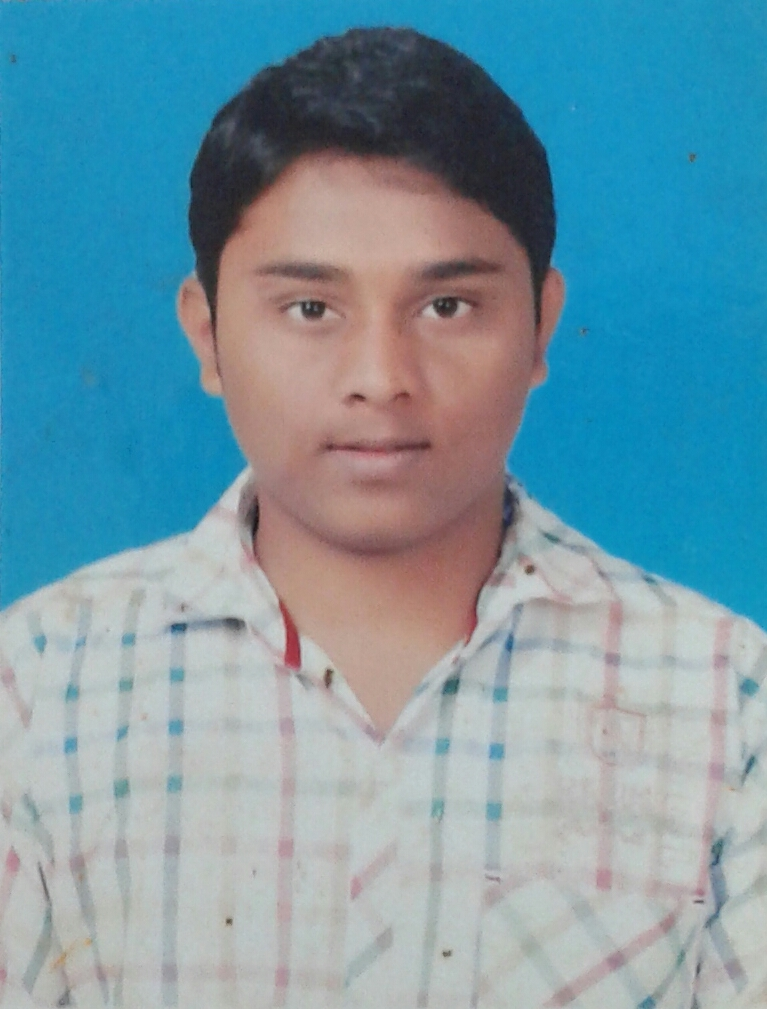
\includegraphics[width=0.2\linewidth,angle=+0]{sushant.jpg}
	\label{fig:sushant}
	\end{flushright}
\end{figure}
\vspace{-4ex}

%Objective

\begin{flushleft}
\textbf{CAREER OBJECTIVE}: To show complete commitment for the walefare of my organization where I can make significant contribution by involvement, keeping my learning objective alive. }
\end{flushleft}

%Education

\begin{flushleft}
\caption{\textbf{EDUCATION:}}\vspace{2ex}
\begin{tabular}{|l|c|c|c|c|r|}  \hline
Degree & College/School & University & Passing Year &  Percentage\\ \hline
B.Tech & Walchand COE, & Shivaji & 2017 & 9.06\\ 
Electrical & Sangli & University & & (CPI) \\ \hline
HSC & Willindon College, Sangli. & - & 2013 & 81.83\\ \hline
SSC & K.P.S.P.,Sangli.& - & 2011 & 92\\ \hline
\end{tabular}
\end{flushleft}

%Projects

\begin{flushleft}
\textbf{PROJECTS:}
\end{flushleft}
\begin{enumerate}
\item Self-regulatory dual dc voltage bus bar system in vehicles using PID control under the guidance of Dr. D R Patil.
\item Image processing based autonomous robot using camera for eYRC+. 
\item Solar powered mobile battery charger.
\item  Automatic street light control. 
\end{enumerate}

%Training and Internship

\begin{flushleft} 
\textbf{TRAINING AND INTERNSHIP :}
\begin{itemize}
\item Industrial Training at �Traction Machine Workshop, Nashik�, from 16th July 2015
to 25th July 2015.
\item Industrial Training at �Tade Power Tech., Sangli�, June 2015.
\end{itemize}
\end{flushleft}

%Technical Skills

\begin{flushleft}
\textbf{TECHNICAL SKILLS : }
\begin{itemize}
\item \textbf{Softwares known:}  Matlab 2015(simulink), Proteus, Keil UVision, MiPower, Zelio-Soft 2 (PLC), Ignition SCADA (novice).
\item Programming in c, python(novice).
\item Controllers worked on: Arduino, 8051, Raspberry-Pi micro-controllers.
\item Analog circuit design.
\item Control system design for power electronic modules.
\end{itemize}
\end{flushleft}

%Soft skills

\begin{flushleft}
\textbf{SOFT SKILLS:}
\begin{enumerate}
\item Leadership.
\item Problem solving. 
\end{enumerate}

%Extra Curricular Activities

\begin{flushleft}
\textbf{EXTRA CURRICULAR ACTIVITIES :}
\begin{itemize}
\item Member of SOFTA, Studants Organization For Technical Activities.
\item Served as volunteer in Robotech committee, in annual technical symposium VISION 2014.
\item Served as Volunteer in First Year Admission Process-2014, WCE, Sangli.
\item  Served as Volunteer in Grduation Ceremony 2014, WCE, Sangli.
\end{itemize}
\end{flushleft}

%Co-curricular Activities

\textbf{CO-CURRICULAR ACTIVITIES : }
\begin{enumerate}
\item \textbf{Winner} in the event Courier Services in E-Yantra+ 2016, a national level robotics competition by IIT-Bombay.
\item \textbf{Winner} in the event Masterminds in TECHNOCRAT-14, a state level technical symposium by EESA, WCE, Sangli.
\item \textbf{Runner Up} in the event StromKries, control system design competition in TECHNOCRAT-15.
\item \textbf{Workshops Attended}\\ 1. PLC and SCADA held by ETA (Educate to Automate).\\
2.Solar and smart energy systems held by Roboversity.
\end{enumerate}

%Personal details and declaration

\textbf{PERSONAL DETAILS:}\\
\vspace{2ex}
Father's Name : Virupaksha Pandurang Bedage.\\
Mother's Name : Jayashri Virupaksha Bedage.\\
Birth date : 6th July, 1995.\\
Gender : Male.\\
Nationality : Indian.\\
Languages known : English, Marathi, Hindi.\\
\vspace{5ex}
\textbf{Declaration:}\\The above information is true to the best of my knowledge and belief.\\
\vspace{5ex}
\textbf{Date:} 25th May 2016
\end{flushleft}
\end {document}
